% This program is free software: you can redistribute it and/or modify
% it under the terms of the GNU AFFERO General Public License as published by
% the Free Software Foundation, either version 3 of the License, or
% (at your option) any later version.
% 
% This program is distributed in the hope that it will be useful,
% but WITHOUT ANY WARRANTY; without even the implied warranty of
% MERCHANTABILITY or FITNESS FOR A PARTICULAR PURPOSE.  See the
% GNU General Public License for more details.
% 
% You should have received a copy of the GNU AFFERO General Public License
% along with this program.  If not, see <https://www.gnu.org/licenses/>.
%
% Copyright (C) 2020 Mo Zhou <cdluminate@gmail.com>
%
\documentclass[9pt,twocolumn,times]{article}
\usepackage{times}
\usepackage[margin=0.9in]{geometry}
\usepackage{tikz}
\usepackage{pgflibraryshapes}
\usetikzlibrary{arrows.meta}
\usepackage{float}
\usepackage{amsmath}
\usepackage{amssymb}
\usepackage{graphicx}
\usepackage{xcolor}
\usepackage{hyperref}
\usepackage{mathtools}
\usepackage{enumitem}
% Source: https://raw.githubusercontent.com/ICLR/Master-Template/master/math_commands.tex
%%%%% NEW MATH DEFINITIONS %%%%%

\usepackage{amsmath,amsfonts,bm}

% Mark sections of captions for referring to divisions of figures
\newcommand{\figleft}{{\em (Left)}}
\newcommand{\figcenter}{{\em (Center)}}
\newcommand{\figright}{{\em (Right)}}
\newcommand{\figtop}{{\em (Top)}}
\newcommand{\figbottom}{{\em (Bottom)}}
\newcommand{\captiona}{{\em (a)}}
\newcommand{\captionb}{{\em (b)}}
\newcommand{\captionc}{{\em (c)}}
\newcommand{\captiond}{{\em (d)}}

% Highlight a newly defined term
\newcommand{\newterm}[1]{{\bf #1}}


% Figure reference, lower-case.
\def\figref#1{figure~\ref{#1}}
% Figure reference, capital. For start of sentence
\def\Figref#1{Figure~\ref{#1}}
\def\twofigref#1#2{figures \ref{#1} and \ref{#2}}
\def\quadfigref#1#2#3#4{figures \ref{#1}, \ref{#2}, \ref{#3} and \ref{#4}}
% Section reference, lower-case.
\def\secref#1{section~\ref{#1}}
% Section reference, capital.
\def\Secref#1{Section~\ref{#1}}
% Reference to two sections.
\def\twosecrefs#1#2{sections \ref{#1} and \ref{#2}}
% Reference to three sections.
\def\secrefs#1#2#3{sections \ref{#1}, \ref{#2} and \ref{#3}}
% Reference to an equation, lower-case.
\def\eqref#1{equation~\ref{#1}}
% Reference to an equation, upper case
\def\Eqref#1{Equation~\ref{#1}}
% A raw reference to an equation---avoid using if possible
\def\plaineqref#1{\ref{#1}}
% Reference to a chapter, lower-case.
\def\chapref#1{chapter~\ref{#1}}
% Reference to an equation, upper case.
\def\Chapref#1{Chapter~\ref{#1}}
% Reference to a range of chapters
\def\rangechapref#1#2{chapters\ref{#1}--\ref{#2}}
% Reference to an algorithm, lower-case.
\def\algref#1{algorithm~\ref{#1}}
% Reference to an algorithm, upper case.
\def\Algref#1{Algorithm~\ref{#1}}
\def\twoalgref#1#2{algorithms \ref{#1} and \ref{#2}}
\def\Twoalgref#1#2{Algorithms \ref{#1} and \ref{#2}}
% Reference to a part, lower case
\def\partref#1{part~\ref{#1}}
% Reference to a part, upper case
\def\Partref#1{Part~\ref{#1}}
\def\twopartref#1#2{parts \ref{#1} and \ref{#2}}

\def\ceil#1{\lceil #1 \rceil}
\def\floor#1{\lfloor #1 \rfloor}
\def\1{\bm{1}}
\newcommand{\train}{\mathcal{D}}
\newcommand{\valid}{\mathcal{D_{\mathrm{valid}}}}
\newcommand{\test}{\mathcal{D_{\mathrm{test}}}}

\def\eps{{\epsilon}}


% Random variables
\def\reta{{\textnormal{$\eta$}}}
\def\ra{{\textnormal{a}}}
\def\rb{{\textnormal{b}}}
\def\rc{{\textnormal{c}}}
\def\rd{{\textnormal{d}}}
\def\re{{\textnormal{e}}}
\def\rf{{\textnormal{f}}}
\def\rg{{\textnormal{g}}}
\def\rh{{\textnormal{h}}}
\def\ri{{\textnormal{i}}}
\def\rj{{\textnormal{j}}}
\def\rk{{\textnormal{k}}}
\def\rl{{\textnormal{l}}}
% rm is already a command, just don't name any random variables m
\def\rn{{\textnormal{n}}}
\def\ro{{\textnormal{o}}}
\def\rp{{\textnormal{p}}}
\def\rq{{\textnormal{q}}}
\def\rr{{\textnormal{r}}}
\def\rs{{\textnormal{s}}}
\def\rt{{\textnormal{t}}}
\def\ru{{\textnormal{u}}}
\def\rv{{\textnormal{v}}}
\def\rw{{\textnormal{w}}}
\def\rx{{\textnormal{x}}}
\def\ry{{\textnormal{y}}}
\def\rz{{\textnormal{z}}}

% Random vectors
\def\rvepsilon{{\mathbf{\epsilon}}}
\def\rvtheta{{\mathbf{\theta}}}
\def\rva{{\mathbf{a}}}
\def\rvb{{\mathbf{b}}}
\def\rvc{{\mathbf{c}}}
\def\rvd{{\mathbf{d}}}
\def\rve{{\mathbf{e}}}
\def\rvf{{\mathbf{f}}}
\def\rvg{{\mathbf{g}}}
\def\rvh{{\mathbf{h}}}
\def\rvu{{\mathbf{i}}}
\def\rvj{{\mathbf{j}}}
\def\rvk{{\mathbf{k}}}
\def\rvl{{\mathbf{l}}}
\def\rvm{{\mathbf{m}}}
\def\rvn{{\mathbf{n}}}
\def\rvo{{\mathbf{o}}}
\def\rvp{{\mathbf{p}}}
\def\rvq{{\mathbf{q}}}
\def\rvr{{\mathbf{r}}}
\def\rvs{{\mathbf{s}}}
\def\rvt{{\mathbf{t}}}
\def\rvu{{\mathbf{u}}}
\def\rvv{{\mathbf{v}}}
\def\rvw{{\mathbf{w}}}
\def\rvx{{\mathbf{x}}}
\def\rvy{{\mathbf{y}}}
\def\rvz{{\mathbf{z}}}

% Elements of random vectors
\def\erva{{\textnormal{a}}}
\def\ervb{{\textnormal{b}}}
\def\ervc{{\textnormal{c}}}
\def\ervd{{\textnormal{d}}}
\def\erve{{\textnormal{e}}}
\def\ervf{{\textnormal{f}}}
\def\ervg{{\textnormal{g}}}
\def\ervh{{\textnormal{h}}}
\def\ervi{{\textnormal{i}}}
\def\ervj{{\textnormal{j}}}
\def\ervk{{\textnormal{k}}}
\def\ervl{{\textnormal{l}}}
\def\ervm{{\textnormal{m}}}
\def\ervn{{\textnormal{n}}}
\def\ervo{{\textnormal{o}}}
\def\ervp{{\textnormal{p}}}
\def\ervq{{\textnormal{q}}}
\def\ervr{{\textnormal{r}}}
\def\ervs{{\textnormal{s}}}
\def\ervt{{\textnormal{t}}}
\def\ervu{{\textnormal{u}}}
\def\ervv{{\textnormal{v}}}
\def\ervw{{\textnormal{w}}}
\def\ervx{{\textnormal{x}}}
\def\ervy{{\textnormal{y}}}
\def\ervz{{\textnormal{z}}}

% Random matrices
\def\rmA{{\mathbf{A}}}
\def\rmB{{\mathbf{B}}}
\def\rmC{{\mathbf{C}}}
\def\rmD{{\mathbf{D}}}
\def\rmE{{\mathbf{E}}}
\def\rmF{{\mathbf{F}}}
\def\rmG{{\mathbf{G}}}
\def\rmH{{\mathbf{H}}}
\def\rmI{{\mathbf{I}}}
\def\rmJ{{\mathbf{J}}}
\def\rmK{{\mathbf{K}}}
\def\rmL{{\mathbf{L}}}
\def\rmM{{\mathbf{M}}}
\def\rmN{{\mathbf{N}}}
\def\rmO{{\mathbf{O}}}
\def\rmP{{\mathbf{P}}}
\def\rmQ{{\mathbf{Q}}}
\def\rmR{{\mathbf{R}}}
\def\rmS{{\mathbf{S}}}
\def\rmT{{\mathbf{T}}}
\def\rmU{{\mathbf{U}}}
\def\rmV{{\mathbf{V}}}
\def\rmW{{\mathbf{W}}}
\def\rmX{{\mathbf{X}}}
\def\rmY{{\mathbf{Y}}}
\def\rmZ{{\mathbf{Z}}}

% Elements of random matrices
\def\ermA{{\textnormal{A}}}
\def\ermB{{\textnormal{B}}}
\def\ermC{{\textnormal{C}}}
\def\ermD{{\textnormal{D}}}
\def\ermE{{\textnormal{E}}}
\def\ermF{{\textnormal{F}}}
\def\ermG{{\textnormal{G}}}
\def\ermH{{\textnormal{H}}}
\def\ermI{{\textnormal{I}}}
\def\ermJ{{\textnormal{J}}}
\def\ermK{{\textnormal{K}}}
\def\ermL{{\textnormal{L}}}
\def\ermM{{\textnormal{M}}}
\def\ermN{{\textnormal{N}}}
\def\ermO{{\textnormal{O}}}
\def\ermP{{\textnormal{P}}}
\def\ermQ{{\textnormal{Q}}}
\def\ermR{{\textnormal{R}}}
\def\ermS{{\textnormal{S}}}
\def\ermT{{\textnormal{T}}}
\def\ermU{{\textnormal{U}}}
\def\ermV{{\textnormal{V}}}
\def\ermW{{\textnormal{W}}}
\def\ermX{{\textnormal{X}}}
\def\ermY{{\textnormal{Y}}}
\def\ermZ{{\textnormal{Z}}}

% Vectors
\def\vzero{{\bm{0}}}
\def\vone{{\bm{1}}}
\def\vmu{{\bm{\mu}}}
\def\vtheta{{\bm{\theta}}}
\def\va{{\bm{a}}}
\def\vb{{\bm{b}}}
\def\vc{{\bm{c}}}
\def\vd{{\bm{d}}}
\def\ve{{\bm{e}}}
\def\vf{{\bm{f}}}
\def\vg{{\bm{g}}}
\def\vh{{\bm{h}}}
\def\vi{{\bm{i}}}
\def\vj{{\bm{j}}}
\def\vk{{\bm{k}}}
\def\vl{{\bm{l}}}
\def\vm{{\bm{m}}}
\def\vn{{\bm{n}}}
\def\vo{{\bm{o}}}
\def\vp{{\bm{p}}}
\def\vq{{\bm{q}}}
\def\vr{{\bm{r}}}
\def\vs{{\bm{s}}}
\def\vt{{\bm{t}}}
\def\vu{{\bm{u}}}
\def\vv{{\bm{v}}}
\def\vw{{\bm{w}}}
\def\vx{{\bm{x}}}
\def\vy{{\bm{y}}}
\def\vz{{\bm{z}}}

% Elements of vectors
\def\evalpha{{\alpha}}
\def\evbeta{{\beta}}
\def\evepsilon{{\epsilon}}
\def\evlambda{{\lambda}}
\def\evomega{{\omega}}
\def\evmu{{\mu}}
\def\evpsi{{\psi}}
\def\evsigma{{\sigma}}
\def\evtheta{{\theta}}
\def\eva{{a}}
\def\evb{{b}}
\def\evc{{c}}
\def\evd{{d}}
\def\eve{{e}}
\def\evf{{f}}
\def\evg{{g}}
\def\evh{{h}}
\def\evi{{i}}
\def\evj{{j}}
\def\evk{{k}}
\def\evl{{l}}
\def\evm{{m}}
\def\evn{{n}}
\def\evo{{o}}
\def\evp{{p}}
\def\evq{{q}}
\def\evr{{r}}
\def\evs{{s}}
\def\evt{{t}}
\def\evu{{u}}
\def\evv{{v}}
\def\evw{{w}}
\def\evx{{x}}
\def\evy{{y}}
\def\evz{{z}}

% Matrix
\def\mA{{\bm{A}}}
\def\mB{{\bm{B}}}
\def\mC{{\bm{C}}}
\def\mD{{\bm{D}}}
\def\mE{{\bm{E}}}
\def\mF{{\bm{F}}}
\def\mG{{\bm{G}}}
\def\mH{{\bm{H}}}
\def\mI{{\bm{I}}}
\def\mJ{{\bm{J}}}
\def\mK{{\bm{K}}}
\def\mL{{\bm{L}}}
\def\mM{{\bm{M}}}
\def\mN{{\bm{N}}}
\def\mO{{\bm{O}}}
\def\mP{{\bm{P}}}
\def\mQ{{\bm{Q}}}
\def\mR{{\bm{R}}}
\def\mS{{\bm{S}}}
\def\mT{{\bm{T}}}
\def\mU{{\bm{U}}}
\def\mV{{\bm{V}}}
\def\mW{{\bm{W}}}
\def\mX{{\bm{X}}}
\def\mY{{\bm{Y}}}
\def\mZ{{\bm{Z}}}
\def\mBeta{{\bm{\beta}}}
\def\mPhi{{\bm{\Phi}}}
\def\mLambda{{\bm{\Lambda}}}
\def\mSigma{{\bm{\Sigma}}}

% Tensor
\DeclareMathAlphabet{\mathsfit}{\encodingdefault}{\sfdefault}{m}{sl}
\SetMathAlphabet{\mathsfit}{bold}{\encodingdefault}{\sfdefault}{bx}{n}
\newcommand{\tens}[1]{\bm{\mathsfit{#1}}}
\def\tA{{\tens{A}}}
\def\tB{{\tens{B}}}
\def\tC{{\tens{C}}}
\def\tD{{\tens{D}}}
\def\tE{{\tens{E}}}
\def\tF{{\tens{F}}}
\def\tG{{\tens{G}}}
\def\tH{{\tens{H}}}
\def\tI{{\tens{I}}}
\def\tJ{{\tens{J}}}
\def\tK{{\tens{K}}}
\def\tL{{\tens{L}}}
\def\tM{{\tens{M}}}
\def\tN{{\tens{N}}}
\def\tO{{\tens{O}}}
\def\tP{{\tens{P}}}
\def\tQ{{\tens{Q}}}
\def\tR{{\tens{R}}}
\def\tS{{\tens{S}}}
\def\tT{{\tens{T}}}
\def\tU{{\tens{U}}}
\def\tV{{\tens{V}}}
\def\tW{{\tens{W}}}
\def\tX{{\tens{X}}}
\def\tY{{\tens{Y}}}
\def\tZ{{\tens{Z}}}


% Graph
\def\gA{{\mathcal{A}}}
\def\gB{{\mathcal{B}}}
\def\gC{{\mathcal{C}}}
\def\gD{{\mathcal{D}}}
\def\gE{{\mathcal{E}}}
\def\gF{{\mathcal{F}}}
\def\gG{{\mathcal{G}}}
\def\gH{{\mathcal{H}}}
\def\gI{{\mathcal{I}}}
\def\gJ{{\mathcal{J}}}
\def\gK{{\mathcal{K}}}
\def\gL{{\mathcal{L}}}
\def\gM{{\mathcal{M}}}
\def\gN{{\mathcal{N}}}
\def\gO{{\mathcal{O}}}
\def\gP{{\mathcal{P}}}
\def\gQ{{\mathcal{Q}}}
\def\gR{{\mathcal{R}}}
\def\gS{{\mathcal{S}}}
\def\gT{{\mathcal{T}}}
\def\gU{{\mathcal{U}}}
\def\gV{{\mathcal{V}}}
\def\gW{{\mathcal{W}}}
\def\gX{{\mathcal{X}}}
\def\gY{{\mathcal{Y}}}
\def\gZ{{\mathcal{Z}}}

% Sets
\def\sA{{\mathbb{A}}}
\def\sB{{\mathbb{B}}}
\def\sC{{\mathbb{C}}}
\def\sD{{\mathbb{D}}}
% Don't use a set called E, because this would be the same as our symbol
% for expectation.
\def\sF{{\mathbb{F}}}
\def\sG{{\mathbb{G}}}
\def\sH{{\mathbb{H}}}
\def\sI{{\mathbb{I}}}
\def\sJ{{\mathbb{J}}}
\def\sK{{\mathbb{K}}}
\def\sL{{\mathbb{L}}}
\def\sM{{\mathbb{M}}}
\def\sN{{\mathbb{N}}}
\def\sO{{\mathbb{O}}}
\def\sP{{\mathbb{P}}}
\def\sQ{{\mathbb{Q}}}
\def\sR{{\mathbb{R}}}
\def\sS{{\mathbb{S}}}
\def\sT{{\mathbb{T}}}
\def\sU{{\mathbb{U}}}
\def\sV{{\mathbb{V}}}
\def\sW{{\mathbb{W}}}
\def\sX{{\mathbb{X}}}
\def\sY{{\mathbb{Y}}}
\def\sZ{{\mathbb{Z}}}

% Entries of a matrix
\def\emLambda{{\Lambda}}
\def\emA{{A}}
\def\emB{{B}}
\def\emC{{C}}
\def\emD{{D}}
\def\emE{{E}}
\def\emF{{F}}
\def\emG{{G}}
\def\emH{{H}}
\def\emI{{I}}
\def\emJ{{J}}
\def\emK{{K}}
\def\emL{{L}}
\def\emM{{M}}
\def\emN{{N}}
\def\emO{{O}}
\def\emP{{P}}
\def\emQ{{Q}}
\def\emR{{R}}
\def\emS{{S}}
\def\emT{{T}}
\def\emU{{U}}
\def\emV{{V}}
\def\emW{{W}}
\def\emX{{X}}
\def\emY{{Y}}
\def\emZ{{Z}}
\def\emSigma{{\Sigma}}

% entries of a tensor
% Same font as tensor, without \bm wrapper
\newcommand{\etens}[1]{\mathsfit{#1}}
\def\etLambda{{\etens{\Lambda}}}
\def\etA{{\etens{A}}}
\def\etB{{\etens{B}}}
\def\etC{{\etens{C}}}
\def\etD{{\etens{D}}}
\def\etE{{\etens{E}}}
\def\etF{{\etens{F}}}
\def\etG{{\etens{G}}}
\def\etH{{\etens{H}}}
\def\etI{{\etens{I}}}
\def\etJ{{\etens{J}}}
\def\etK{{\etens{K}}}
\def\etL{{\etens{L}}}
\def\etM{{\etens{M}}}
\def\etN{{\etens{N}}}
\def\etO{{\etens{O}}}
\def\etP{{\etens{P}}}
\def\etQ{{\etens{Q}}}
\def\etR{{\etens{R}}}
\def\etS{{\etens{S}}}
\def\etT{{\etens{T}}}
\def\etU{{\etens{U}}}
\def\etV{{\etens{V}}}
\def\etW{{\etens{W}}}
\def\etX{{\etens{X}}}
\def\etY{{\etens{Y}}}
\def\etZ{{\etens{Z}}}

% The true underlying data generating distribution
\newcommand{\pdata}{p_{\rm{data}}}
% The empirical distribution defined by the training set
\newcommand{\ptrain}{\hat{p}_{\rm{data}}}
\newcommand{\Ptrain}{\hat{P}_{\rm{data}}}
% The model distribution
\newcommand{\pmodel}{p_{\rm{model}}}
\newcommand{\Pmodel}{P_{\rm{model}}}
\newcommand{\ptildemodel}{\tilde{p}_{\rm{model}}}
% Stochastic autoencoder distributions
\newcommand{\pencode}{p_{\rm{encoder}}}
\newcommand{\pdecode}{p_{\rm{decoder}}}
\newcommand{\precons}{p_{\rm{reconstruct}}}

\newcommand{\laplace}{\mathrm{Laplace}} % Laplace distribution

\newcommand{\E}{\mathbb{E}}
\newcommand{\Ls}{\mathcal{L}}
\newcommand{\R}{\mathbb{R}}
\newcommand{\emp}{\tilde{p}}
\newcommand{\lr}{\alpha}
\newcommand{\reg}{\lambda}
\newcommand{\rect}{\mathrm{rectifier}}
\newcommand{\softmax}{\mathrm{softmax}}
\newcommand{\sigmoid}{\sigma}
\newcommand{\softplus}{\zeta}
\newcommand{\KL}{D_{\mathrm{KL}}}
\newcommand{\Var}{\mathrm{Var}}
\newcommand{\standarderror}{\mathrm{SE}}
\newcommand{\Cov}{\mathrm{Cov}}
% Wolfram Mathworld says $L^2$ is for function spaces and $\ell^2$ is for vectors
% But then they seem to use $L^2$ for vectors throughout the site, and so does
% wikipedia.
\newcommand{\normlzero}{L^0}
\newcommand{\normlone}{L^1}
\newcommand{\normltwo}{L^2}
\newcommand{\normlp}{L^p}
\newcommand{\normmax}{L^\infty}

\newcommand{\parents}{Pa} % See usage in notation.tex. Chosen to match Daphne's book.

\DeclareMathOperator*{\argmax}{arg\,max}
\DeclareMathOperator*{\argmin}{arg\,min}

\DeclareMathOperator{\sign}{sign}
\DeclareMathOperator{\Tr}{Tr}
\let\ab\allowbreak


\title{Computation Graph Spickzettel}
\author{Mo Zhou\\\small\texttt{<cdluminate@gmail.com>}\\
License: AGPL-3.0}

\begin{document}

\maketitle
\tableofcontents
\newpage

\section{Conventions}

Vectors are column vectors by default.
We follow the naming convention of BLAS/LAPACK for linear algebra operations.
Vecotr, Matrix, Tensor shapes are annotated under the corresponding symbols.
Throughout the whole document, $L$ denotes any loss function (\emph{i.e.},
objective function) of interest.

\section{Automatic Differentiation}

\section{Atomic Modules}

\subsection{Level1: Vector-Vector Ops}

\begin{enumerate}[leftmargin=*]
\item \textbf{Identity} (I)
\begin{equation}
	\underset{(m)}{\vx} = \underset{(m)}{\vy}
\end{equation}
\begin{center}
	\resizebox{0.618\columnwidth}{!}{%
		% This program is free software: you can redistribute it and/or modify
% it under the terms of the GNU AFFERO General Public License as published by
% the Free Software Foundation, either version 3 of the License, or
% (at your option) any later version.
%
% This program is distributed in the hope that it will be useful,
% but WITHOUT ANY WARRANTY; without even the implied warranty of
% MERCHANTABILITY or FITNESS FOR A PARTICULAR PURPOSE.  See the
% GNU General Public License for more details.
%
% You should have received a copy of the GNU AFFERO General Public License
% along with this program.  If not, see <https://www.gnu.org/licenses/>.
%
% Copyright (C) 2020 Mo Zhou <cdluminate@gmail.com>
%
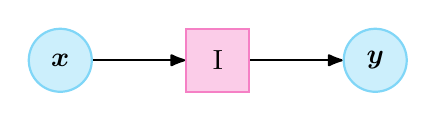
\begin{tikzpicture}[thick,minimum size=8mm]
	\node (x) at (0,0) [circle,draw=cyan!50,fill=cyan!20] {$\vx$};
	\node (ident) at (2,0) [rectangle,draw=magenta!50,fill=magenta!20] {I};
	\node (y) at (4,0) [circle,draw=cyan!50,fill=cyan!20] {$\vy$};
	\draw [-{Latex[round]}] (x) -- (ident);
	\draw [-{Latex[round]}] (ident) -- (y);
\end{tikzpicture}

	}
\end{center}
\begin{equation}
	\underset{(m)}{\frac{\partial L}{\partial \vx}} =
	\underset{(m)}{\frac{\partial L}{\partial \vy}}
\end{equation}

\item \textbf{Transpose} (T)
\begin{equation}
	\underset{(1\times m)}{\vx^T} = \underset{(1\times m)}{\vy}
\end{equation}
\begin{center}
	\resizebox{0.618\columnwidth}{!}{%
		% This program is free software: you can redistribute it and/or modify
% it under the terms of the GNU AFFERO General Public License as published by
% the Free Software Foundation, either version 3 of the License, or
% (at your option) any later version.
%
% This program is distributed in the hope that it will be useful,
% but WITHOUT ANY WARRANTY; without even the implied warranty of
% MERCHANTABILITY or FITNESS FOR A PARTICULAR PURPOSE.  See the
% GNU General Public License for more details.
%
% You should have received a copy of the GNU AFFERO General Public License
% along with this program.  If not, see <https://www.gnu.org/licenses/>.
%
% Copyright (C) 2020 Mo Zhou <cdluminate@gmail.com>
%
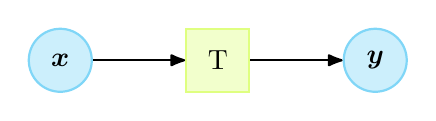
\begin{tikzpicture}[thick,minimum size=8mm]
	\node (x) at (0,0) [circle,draw=cyan!50,fill=cyan!20] {$\vx$};
	\node (trans) at (2,0) [rectangle,draw=lime!50,fill=lime!20] {T};
	\node (y) at (4,0) [circle,draw=cyan!50,fill=cyan!20] {$\vy$};
	\draw [-{Latex[round]}] (x) -- (trans);
	\draw [-{Latex[round]}] (trans) -- (y);
\end{tikzpicture}

	}
\end{center}
\begin{equation}
	\underset{(m)}{\frac{\partial L}{\partial \vx}} =
	\underset{(m)}{\Big(\frac{\partial L}{\partial \vy}\Big)^T}
\end{equation}

\item \textbf{Addition} (Add)
\begin{equation}
	\underset{(m)}{\vx} + \underset{(m)}{\vz} =
	\underset{(m)}{\vy}
\end{equation}
\begin{center}
	\resizebox{0.618\columnwidth}{!}{%
		% This program is free software: you can redistribute it and/or modify
% it under the terms of the GNU AFFERO General Public License as published by
% the Free Software Foundation, either version 3 of the License, or
% (at your option) any later version.
%
% This program is distributed in the hope that it will be useful,
% but WITHOUT ANY WARRANTY; without even the implied warranty of
% MERCHANTABILITY or FITNESS FOR A PARTICULAR PURPOSE.  See the
% GNU General Public License for more details.
%
% You should have received a copy of the GNU AFFERO General Public License
% along with this program.  If not, see <https://www.gnu.org/licenses/>.
%
% Copyright (C) 2020 Mo Zhou <cdluminate@gmail.com>
%
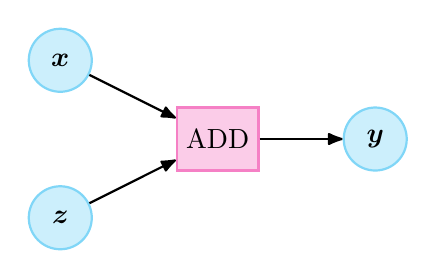
\begin{tikzpicture}[thick,minimum size=8mm]
	\node (x) at (0,0) [circle,draw=cyan!50,fill=cyan!20] {$\vx$};
	\node (z) at (0,-2) [circle,draw=cyan!50,fill=cyan!20] {$\vz$};
	\node (add) at (2,-1) [rectangle,draw=magenta!50,fill=magenta!20] {ADD};
	\node (y) at (4,-1) [circle,draw=cyan!50,fill=cyan!20] {$\vy$};
	\draw [-{Latex[round]}] (x) -- (add);
	\draw [-{Latex[round]}] (z) -- (add);
	\draw [-{Latex[round]}] (add) -- (y);
\end{tikzpicture}

	}
\end{center}
\begin{align}
	\mJ &= \underset{(m\times m)}{\mI} \\
	\underset{(m)}{\frac{\partial L}{\partial \vx}} &=
	\underset{(m)}{\frac{\partial L}{\partial \vy}} \\
	\underset{(m)}{\frac{\partial L}{\partial \vz}} &=
	\underset{(m)}{\frac{\partial L}{\partial \vy}}
\end{align}

\item \textbf{Element-wise Multiplication} (Mul)

\item \textbf{Dot Product} (Dot)

\item \textbf{Element-wise Inverse} (Inv)

\item \textbf{L-2 Norm} (L-2)

\item \textbf{Rectified Linear Unit} (ReLU)

\item \textbf{Sigmoid} ($\sigma$)
\end{enumerate}

\subsection{Level2: Matrix-Vector Ops}

\begin{enumerate}[leftmargin=*]
\item \textbf{GEneral Matrix-Vector multiplication} (GEMV)
\begin{equation}
	\underset{(m\times k)}{\mW} \cdot \underset{(k)}{\vx} =
	\underset{(m)}{\vy}
\end{equation}
\begin{center}
	\resizebox{0.618\columnwidth}{!}{%
		% This program is free software: you can redistribute it and/or modify
% it under the terms of the GNU AFFERO General Public License as published by
% the Free Software Foundation, either version 3 of the License, or
% (at your option) any later version.
%
% This program is distributed in the hope that it will be useful,
% but WITHOUT ANY WARRANTY; without even the implied warranty of
% MERCHANTABILITY or FITNESS FOR A PARTICULAR PURPOSE.  See the
% GNU General Public License for more details.
%
% You should have received a copy of the GNU AFFERO General Public License
% along with this program.  If not, see <https://www.gnu.org/licenses/>.
%
% Copyright (C) 2020 Mo Zhou <cdluminate@gmail.com>
%
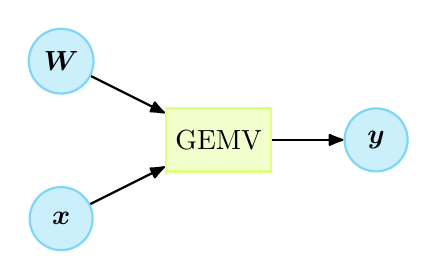
\begin{tikzpicture}[thick,minimum size=8mm]
	\node (w) at (0,0) [circle,draw=cyan!50,fill=cyan!20] {$\mW$};
	\node (x) at (0,-2) [circle,draw=cyan!50,fill=cyan!20] {$\vx$};
	\node (gemv) at (2,-1) [rectangle,draw=lime!50,fill=lime!20] {GEMV};
	\node (y) at (4,-1) [circle,draw=cyan!50,fill=cyan!20] {$\vy$};
	\draw [-{Latex[round]}] (w) -- (gemv);
	\draw [-{Latex[round]}] (x) -- (gemv);
	\draw [-{Latex[round]}] (gemv) -- (y);
\end{tikzpicture}

	}
\end{center}
\begin{align}
	\underset{(m\times k)}{\frac{\partial L}{\partial\mW}} &=
	\underset{(m)}{\frac{\partial L}{\partial\vy}} \cdot
	\underset{(1\times k)}{\vx^T}\\
	\underset{(k)}{\frac{\partial L}{\partial\vx}} &=
	\underset{(k\times m)}{\mW^T} \cdot
	\underset{(m)}{\frac{\partial L}{\partial \vy}}
\end{align}

\end{enumerate}

\subsection{Level3: Matrix-Matrix Ops}

\begin{enumerate}[leftmargin=*]
\item \textbf{GEneral Matrix-Matrix multiplication} (GEMM)
\begin{equation}
	\underset{(m\times k)}{\mW} \cdot
	\underset{(k\times n)}{\mX} =
	\underset{(m\times n)}{\mY}
\end{equation}
\begin{center}
	\resizebox{0.618\columnwidth}{!}{%
		% This program is free software: you can redistribute it and/or modify
% it under the terms of the GNU AFFERO General Public License as published by
% the Free Software Foundation, either version 3 of the License, or
% (at your option) any later version.
%
% This program is distributed in the hope that it will be useful,
% but WITHOUT ANY WARRANTY; without even the implied warranty of
% MERCHANTABILITY or FITNESS FOR A PARTICULAR PURPOSE.  See the
% GNU General Public License for more details.
%
% You should have received a copy of the GNU AFFERO General Public License
% along with this program.  If not, see <https://www.gnu.org/licenses/>.
%
% Copyright (C) 2020 Mo Zhou <cdluminate@gmail.com>
%
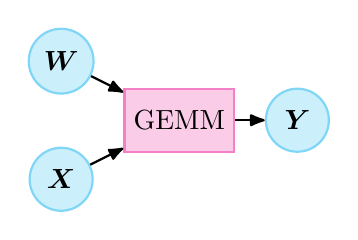
\begin{tikzpicture}[thick,minimum size=8mm]
	\node (w) at (0,0) [circle,draw=cyan!50,fill=cyan!20] {$\mW$};
	\node (x) at (0,-1.5) [circle,draw=cyan!50,fill=cyan!20] {$\mX$};
	\node (gemm) at (1.5,-0.75) [rectangle,draw=magenta!50,fill=magenta!20] {GEMM};
	\node (y) at (3,-0.75) [circle,draw=cyan!50,fill=cyan!20] {$\mY$};
	\draw [-{Latex[round]}] (w) -- (gemm);
	\draw [-{Latex[round]}] (x) -- (gemm);
	\draw [-{Latex[round]}] (gemm) -- (y);
\end{tikzpicture}

	}
\end{center}
\begin{align}
	\underset{(m\times k)}{\frac{\partial L}{\partial\mW}} &=
	\underset{(m\times n)}{\frac{\partial L}{\partial\mY}} \cdot
	\underset{(n,k)}{\mX^T}\\
	\underset{(k\times n)}{\frac{\partial L}{\partial\mX}} &=
	\underset{(k\times m)}{\mW^T} \cdot
	\underset{(m\times n)}{\frac{\partial L}{\partial \mY}}
\end{align}

\item \textbf{2-D Convolution} (Conv2d)
\end{enumerate}

\section{Network Layers}

\begin{enumerate}[leftmargin=*]
\item \textbf{Affine Transformation Layer} (Affine)

\item \textbf{Mean Square Error} (MSE)
\begin{equation}
	\frac{1}{H} \sum_{i=1}^H
	\|\underset{(n)}{\vx_i} - \underset{(n)}{\hat{\vx}_i} \|_2^2
	= \underset{(1)}{L} 
\end{equation}
\begin{figure}[h]
	\centering
	\resizebox{0.618\columnwidth}{!}{%
		% This program is free software: you can redistribute it and/or modify
% it under the terms of the GNU AFFERO General Public License as published by
% the Free Software Foundation, either version 3 of the License, or
% (at your option) any later version.
%
% This program is distributed in the hope that it will be useful,
% but WITHOUT ANY WARRANTY; without even the implied warranty of
% MERCHANTABILITY or FITNESS FOR A PARTICULAR PURPOSE.  See the
% GNU General Public License for more details.
%
% You should have received a copy of the GNU AFFERO General Public License
% along with this program.  If not, see <https://www.gnu.org/licenses/>.
%
% Copyright (C) 2020 Mo Zhou <cdluminate@gmail.com>
%
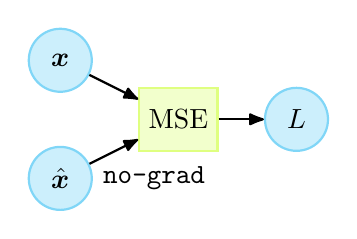
\begin{tikzpicture}[thick,minimum size=8mm]
	\node (x) at (0,0) [circle,draw=cyan!50,fill=cyan!20] {$\vx$};
	\node (hx) at (0,-1.5) [circle,draw=cyan!50,fill=cyan!20,label=right:{\tt no-grad}] {$\hat{\vx}$};
	\node (mse) at (1.5,-0.75) [rectangle,draw=lime!50,fill=lime!20] {MSE};
	\node (l) at (3,-0.75) [circle,draw=cyan!50,fill=cyan!20] {$L$};
	\draw [-{Latex[round]}] (x) -- (mse);
	\draw [-{Latex[round]}] (hx) -- (mse);
	\draw [-{Latex[round]}] (mse) -- (l);
\end{tikzpicture}

	}
	\caption{MSE: $\frac{1}{H} \sum_{i=1}^H \|\vx_i - \hat{\vx}_i\|_2^2 = L$.}
\end{figure}

\item \textbf{Softmax Layer} (Softmax)

\item \textbf{Batch Normalization} (BN)
\end{enumerate}

\section{Networks}

\subsection{Convolutional Neural Networks}

\subsection{Recurrent Neural Networks}

\end{document}
